\section{Ejercicio 3}

% El nuevo problema que tienen Marty y el Doc es que ahora no se ponen de
% acuerdo en qué estructura quı́mica deben utilizar para armar el condensador
% de flujos. Marty, a partir de las propiedades atómicas, ha obtenido una
% constante n y está seguro de que la solución que están buscando debe ser un
% grafo de a lo sumo n vértices (o como él lo dice, un subgrafo de algún Kn),
% mientras que el Doc ha estudiado las caracterı́sticas moleculares e insiste
% con que debe ser un subgrafo de un cografo dado. Por las dudas, y para
% evitar más conflictos entre ellos, quieren cumplir con ambas
% especificaciones, siempre maximizando la cantidad de aristas, dado que éste
% es el punto clave para su funcionamiento dentro del condensador. Por eso les
% pedimos que los ayuden diseñando e implementando un algoritmo exacto para
% MCS que tenga complejidad temporal polinomial para el caso en el que G1 es
% un cografo y G2 es un grafo completo y desarrollen los siguientes puntos que
% avalen la solución encontrada (si estamos hablando de viajar en el tiempo,
% no hay margen de error posible):
% a) Explicar detalladamente el algoritmo implementado.
% b) Calcular el orden de complejidad temporal de peor caso del algoritmo.
% c) Realizar una experimentación que permita observar los tiempos de
%    ejecución del algoritmo en función del tamaño de entrada.

\subsection{Introducción}
En este ejercicio, se busca encontrar un algoritmo exacto para resolver, en
tiempo polinomial, el problema del \acr{MCS} entre dos grafos cuando uno de
ellos es un grafo completo y el otro es un \emph{cografo}. La clase de los
cografos, o grafos reducibles por complemento, se define recursivamente y
consiste exactamente en los grafos que pueden construirse según alguna de las
siguientes reglas:
\begin{enumerate}
    \item Un nodo aislado ($K_1$) es un cografo.
    \item La unión de dos o más cografos es un cografo.
    \item El complemento de un cografo es un cografo.
\end{enumerate}

Es posible demostrar (\cite{corneil}, Corneil et al.) que todo cografo
admite una representación mediante un árbol enraizado, que se conoce como
coárbol (o \emph{cotree}) del mismo. Existen diferentes variantes de esta
representación, pero en todas ellas las hojas del árbol corresponden a los
nodos del grafo, mientras que los nodos internos representan el cografo que se
obtiene aplicando una determinada operación a los cografos relativos a sus
nodos hijos. Así, la raíz del coárbol se corresponde con el cografo completo
que se busca representar.

% Para obtener esta representación se parte de que todo cografo, o bien es una
% unión disjunta de cografos, o su complemento lo es. De esto se sigue que
% todo cografo puede reducirse a un conjunto de nodos aislados complementando
% de forma sucesiva sus componentes conexas (de allí que a estos grafos se los
% conozca como \emph{reducibles por complemento}). Esto equivale a decir que
% puede darse una forma iterativa para construir cualquier cografo a partir de
% sus nodos; se comienza considerando todos ellos como grafos disjuntos, y
% luego se conectan estos grafos iterativamente computando en cada paso el
% complemento de la unión de algunos de ellos. Dado un cografo cualquiera, su
% coárbol no es más que la representación de este proceso mediante un árbol:
% las hojas del mismo corresponden a los nodos del cografo, y cada nodo
% interno representa el complemento de la unión de los cografos
% correspondientes a sus hijos. El cografo en sí mismo es representado la raíz
% del árbol.

En este trabajo, las dos operaciones que se utilizarán para etiquetar los
nodos internos de un coárbol provienen de una definición alternativa y
equivalente de cografo: un grafo es un cografo si y solo si puede obtenerse a
partir de nodos aislados mediante la aplicación sucesiva de la unión disjunta
($\cup$) y el \emph{join} ($\times$). Esta última operación se define de la
siguiente forma: dados $G_1, \dots, G_k$ grafos, el \emph{join} entre ellos es
el grafo $G_1 \times \dots \times G_k = \left((G_1)\comp \cup
\dots \cup (G_k)\comp\right)\comp$. Una forma más intuitiva de pensar el
\emph{join} entre grafos es partir de la unión disjunta entre ellos, y agregar
todas las aristas cuyos extremos se encontraban en grafos distintos.

Otra consideración a tener en cuenta es que, para simplificar la
implementación, se utilizarán coárboles estrictamente binarios; es decir,
cada nodo interno representará una operación entre exactamente dos cografos.
Esto no resulta problemático, ya que tanto la unión como el \emph{join} entre
grafos son operaciones asociativas.

\begin{figure}[htbp]
    \centering
    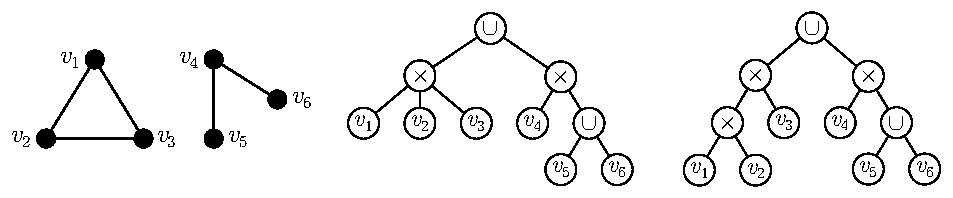
\includegraphics{imagenes/cografos-ejemplo-coarbol.pdf}
    \caption{Ejemplo de un cografo, su coárbol correspondiente, y la
    representación estrictamente binaria del mismo.}
    \label{fig:cografos:ejemplo-coarbol}
\end{figure}

\subsection{Resolución algorítmica}
Sean $G_1 = K_{N_1}$ un grafo completo de $N_1$ nodos (que tendrá por lo tanto
$M_1 = \frac{N_1 \times (N_1 - 1)}{2}$ aristas), y $G_2$ un cografo con $N_2$
nodos y $M_2$ aristas. A la hora de resolver el problema de encontrar el \acr
{MCS} entre $G_1$ y $G_2$, pueden distinguirse estos dos casos:
\begin{enumerate}
    \item $N_1 \geq N_2$. Dado que $G_1$ es un grafo completo, todo
    subgrafo que tenga $N_1$ o menos aristas, y en particular $G_2$,
    es isomorfo a algún subgrafo de $G_1$. Como, trivialmente, $G_2$ es
    isomorfo a sí mismo, basta tomar $G_2$ como solución del problema.
    \item $N_1 < N_2$. En este caso, sea $H$ un grafo isomorfo a algún
    subgrafo de $G_2$; $H$ resultará isomorfo a algún subgrafo de $G_1$ si
    y solo si su cantidad de nodos es menor o igual que $N_1$. Si $H$ tiene
    menos de $N_1$ nodos, puede extenderse a algún grafo $\tilde{H} \supseteq
    H$ que tenga $N_1$ nodos y también sea isomorfo a un subgrafo de $G_2$.
    Es directo que $\tilde{H}$ resulta isomorfo a algún subgrafo de $G_1$ y
    que su cantidad de aristas es mayor o igual que la de $H$. Entonces, si
    $H$ era solución óptima de \acr{MCS}, claramente $\tilde{H}$ también lo
    es. De esto se sigue que para resolver este caso del problema, basta con
    tomar un subgrafo de $G_2$ que tenga exactamente $N_1$ nodos y maximice la
    cantidad de aristas.
\end{enumerate}

Dado que la resolución del primer caso es trivial, durante el resto de esta
sección se asumirá que $N_1 < N_2$. Se llamará $K = N_1$, $G = G_2$, $N = N_2$
y $M = M_2$, y se explicará la solución planteada al problema de encontrar un
subgrafo de un cografo $G$ que tenga exactamente $K$ vértices y cantidad de
aristas máxima.

En general, el problema de determinar para un grafo dado el subgrafo con
determinada cantidad de vértices que maximice la cantidad de aristas es
NP-completo, y por lo tanto, no se conoce un algoritmo eficiente para
resolverlo. No obstante, aprovechando la hipótesis de que $G$ es un cografo,
es posible solucionar el problema en tiempo polinomial.

La solución propuesta tiene dos etapas. En primer lugar, se crea el coárbol
binario de $G$, y luego, utilizando la técnica de programación dinámica, se
aprovecha esta representación para obtener el subgrafo buscado.

\subsubsection{Resultados preliminares}
A continuación, se demostrarán una serie de resultados que serán necesarios
para asegurar la correctitud de los algoritmos presentados más adelante.

\subsubsection{Construcción del coárbol}
Para construir el coárbol correspondiente a un cografo dado, se aprovecha la
en cografos de menor tamaño hasta obtener un conjunto de vértices aislados.
El algoritmo admite una sencilla formulación recursiva: si el cografo consiste
en un vértice aislado, el coárbol tendrá un único nodo representando este
vértice. En caso contrario, el cografo será la unión o el \emph{join} de dos
cografos; el coárbol que lo represente tendrá como raíz un nodo etiquetado con
esa operación, del cual colgarán los coárboles correspondientes a los dos
cografos sobre los cuales esta se aplica.

\subsubsection{Búsqueda del subgrafo máximo}
Para encontrar el subgrafo de $G$ con $K < N$ nodos y máxima cantidad de
aristas, se diseñó un algoritmo utilizando la técnica de programación
dinámica. El esquema detrás de la formulación recursiva de este algoritmo es
la siguiente:

\begin{enumerate}
    \item Si $K = 0$, la solución del algoritmo es un grafo sin nodos ni
    aristas.
    \item Si $K > 0$ y $G = K_1$, es decir, un nodo aislado, la solución es
    $K_1$.
    \item Si $G \neq K_1$, entonces existen dos cografos $G_1$ y $G_2$ tales
    que $G = G_1 \times G_2$ o $G = G_1 \cup G_2$. En tal caso, la solución
    $H$ del problema tendrá algunos de sus nodos en $G_1$ y el resto en $G_2$.
    Entonces, según la operación con la que se obtenga $G$ a partir de $G_1$ y
    $G_2$, tenemos que $H = H_1 \times H_2$ o $H = H_1 \cup H_2$, donde
    $H_1$ y $H_2$ son los subgrafos inducidos en $G$ por los nodos de $H$ que
    pertenecen a $G_1$ y a $G_2$, respectivamente.
\end{enumerate}

\[
    \operatorname{MCS}(G, K) = \begin{cases}
        (\varnothing, \varnothing) & \text{si } K = 0 \\
        K_1 & \text{si } G \text{ es un nodo aislado} \\
        \displaystyle \argmax_{H \in S(G, K)}(\#E(H)) & \text{si } G = (G_1
        \cup G_2) \text{ o } G = (G_1 \times G_2) \\
    \end{cases}
\]

donde

\[
    S(G, K) = \begin{cases}
        \lbrace \operatorname{MCS}(G_1, k) \cup \operatorname{MCS}(G_2, K -
        k) \ \vert\ 0 \leq k \leq K \rbrace & \text{si } G = (G_1 \cup G_2) \\
        \lbrace \operatorname{MCS}(G_1, k) \times \operatorname{MCS}(G_2, K -
        k) \ \vert\ 0 \leq k \leq K \rbrace & \text{si } G = (G_1 \times G_2)
    \end{cases}
\]

\begin{algorithm}[H]
    % \caption{Búsqueda del }
    \Input{Un cografo $G = (V, E)$ con $N$ nodos y $M$ aristas, y un natural
        $K < N$.}
    \Output{Un subgrafo $H \subseteq G$ con $K$ nodos que maximice la cantidad
        de aristas.}

    $cotree$ $\gets$ cotree correspondiente a $G$ \;
    $DP$ $\gets$ grilla de dimensiones $(2 \times N - 1) \times K$, donde \;
    cada fila representa a uno de los vértices del coárbol de $G$, y cada \;
    columna,
    \Return{($DP_{N,M}$, $camino$)}
\end{algorithm}


El algoritmo planteado para la búsqueda del máximo subgrafo


\subsection{Detalles implementativos}

\subsection{Complejidad}
Defino $n_1$ la cantiadad de nodos de $g_1$ (cografo) y $m_1$ la cantiadad de aristas, 
$n_2$ la cantidad de nodos del $g_2$ ($K_n$) 

Armar el cotree tiene una complejidad $O(n_1(n_1 + m_1))$ , hacer el DP que calcula la solucion $O(n_1 * (n_2)^2 )$

En total el algoritmo termina teniendo una complejidad de $O(n_1((n_1 + m_1) + (n_2)^2 ))$

\subsection{Experimentación}

    

    Para la solucion del DP se hicieron tres experimentos:

    \begin{enumerate}
        \item Se Varia los nodos del cografo ($n_1$) y se fija el $K_n$ en 100 nodos, se varia la cantidad de aristas del cografo para ver como afecta al solver DP . Se esperan funciones lineales diferriendo en una constante, dependiendo de como este conectado el cografo. Con este experimento se espera probar la dependencia lineal de $n_1$.
        \item Se varia el cografo en $n$, siendo el cografo un $K_n$  y el segundo grafo en $K_{n/2}$. Se espera funcion cubica , con la cual se pretende mostrar la dependecia cuadratica de $n_2$ y confirmar la depencia lineal de $n_1$.
        \item Se varia el cografo en $n$, siendo el cografo un $K_n$  y el segundo grafo en $K_{log(n)}$. Se espera una funcion de la pint $xlog^2(x)$ , con la cual se pretende mostrar la dependecia cuadratica de $n_2$ y confirmar la depencia lineal de $n_1$.
    \end{enumerate}

    Para la creacion del coarbol se hicieron tres experimentos:

    \begin{enumerate}

        \item Se toma la union de $K_1$, con lo cual se fija la cantidad de aristas en $0$ ($m_1$) y se varia la cantidad de nodos del cografo($n_1$). Se espera una funcion cuadratica, con la cual se quiere mostrar la depencia cuadratica de $n_1$.
        \item Se toma la union de $K_3$, cada 3 nuevos nodos hay 3 nuevas aristas , logrando una dependia lineal $m_1 = n_1$. Se espera una funcion cuadratica con una constante más alta que la union de $K_1$. Con lo cual se espera probar parcialmente la influencia de $m_1$ y confirmar la dependecia cuadratica de $n_1$
        \item Se toma un $K_n$ , con lo cual se tiene una dependencia cuadratica $m_1 = n_1(n_1 - 1)$. Se espera una funcion cuadratica, con la cual se pretende mostrar la influencia de $m_2$.

    \end{enumerate}


    Se experimentó con la creacion del cotree y con la solucion del DP por separado para 
     tener un mayor control de las variables.

 
   \subsubsection{ Experimentos con el solver DP}


    
    \begin{figure}[H]
        \centering
        \begin{tikzpicture}
            \begin{axis}[
                    title={},
                    xlabel={Se Varia los nodos del cografo ($n_1$) y se fija el $K_n$ en 100 nodos.},
                    ylabel={Tiempo de ejecución (nanosegundos)},
                    scaled x ticks=false,
                    scaled y ticks=false,
                    enlargelimits=0.05,
                    width=0.5\textwidth,
                    height=0.5\textwidth,
                    legend pos=north west,
                    legend cell align=left,
                    xmin=100
                ]
                \addplot[color=black] table[x index=0,y index=1]{../exp/ej3/cograph_kn_dp};
                \addplot[color=blue] table[x index=0,y index=1]{../exp/ej3/cograph_k1_union_dp};
                \addplot[color=violet] table[x index=0,y index=1]{../exp/ej3/cograph_k10_union_dp};

                \addplot[color=red] table[x index=0, y expr={ 500000 * (x) }]{../exp/ej3/cograph_kn_dp};
                \legend{$T_{k_n}$,$T_{k_1}$,$T_{k_{10}}$,$ C * x $}
            \end{axis}
        \end{tikzpicture}
        \caption{Se ejecuto la resolucion del DP. como $n_2 = 100$ nos queda una complejidad $O(n1* 100^2)$ = $O(n1)$ }
        \label{fig:exp3:var-nym-base}
    \end{figure}

    Se puede ver que la constante depende del la familia del grafo , ya que $T_{k_n}$ y $T_{k_1}$ tiene una constante muy parecida , ya que uno es el complemento del otro. Queda ver con diversas familias de cografos para ver como afecta al la creacion de coarboles.Se puede esperar mientras más balanceado sea el coarbol más grande sera la constante, ya que en cada paso tendria que probar hijos izquierdos por hijos derechos en el DP.

    

     \begin{figure}[H]
        \centering
        \begin{tikzpicture}
            \begin{axis}[
                    title={},
                    xlabel={Se Varia los nodos del cografo ($n_1$) y se fija el $K_n$ en 100 nodos.},
                    ylabel={Tiempo de ejecución (nanosegundos)},
                    scaled x ticks=false,
                    scaled y ticks=false,
                    enlargelimits=0.05,
                    width=0.5\textwidth,
                    height=0.5\textwidth,
                    legend pos=north west,
                    legend cell align=left,
                    xmin=100
                ];
                \addplot[color=black] table[x index=0,y expr={\thisrowno{1}/(x)} ]{../exp/ej3/cograph_kn_dp};
                \addplot[color=blue] table[x index=0,y expr={\thisrowno{1}/(x)} ]{../exp/ej3/cograph_k1_union_dp};
                \addplot[color=violet] table[x index=0,y expr={\thisrowno{1}/(x)} ]{../exp/ej3/cograph_k10_union_dp};
                \addplot[color=red] table[x index=0, y expr={ 500000 }]{../exp/ej3/cograph_kn_dp};
                \legend{$T_{k_n}$,$T_{k_1}$,$T_{k_{10}}$,$ C * x $}
            \end{axis}
        \end{tikzpicture}
        \caption{Se divide por $n_1$, para mostrar que $C =  500000$ lo acota.}
        \label{fig:exp3:var-nym-base}
    \end{figure}


    


    \begin{figure}[H]
        \centering
        \begin{tikzpicture}
            \begin{axis}[
                    title={},
                    xlabel={Se varia los nodos del cografo, siendo  un $K_n$  y el segundo grafo tiene le mitad de nodos.},
                    ylabel={Tiempo de ejecución (nanosegundos)},
                    scaled x ticks=false,
                    scaled y ticks=false,
                    enlargelimits=0.05,
                    width=0.5\textwidth,
                    height=0.5\textwidth,
                    legend pos=north west,
                    legend cell align=left,
                    xmin=0
                ]
                \addplot[color=black] table[x index=0,y index=1]{../exp/ej3/cograph_kn_and_k_n_div_2_dp};
                \addplot[color=red] table[x index=0, y expr={ 10 * (x*x*x) }]{../exp/ej3/cograph_kn_and_k_n_div_2_dp};
                \legend{$T_{k_n}$,$ C * x^3 $}
            \end{axis}
        \end{tikzpicture}
        \caption{Se ejecuto la resolucion del DP. como $n_2 = n_1/2$ nos queda una complejidad $O(n_1* (n_1/2)^2)$ = $O(n_1^3)$}
        \label{fig:exp3:var-nym-base}
    \end{figure}

    \begin{figure}[H]
        \centering
        \begin{tikzpicture}
            \begin{axis}[
                    title={},
                    xlabel={Se varia los nodos del cografo, siendo  un $K_n$  y el segundo grafo tiene le mitad de nodos.},
                    ylabel={Tiempo de ejecución (nanosegundos)},
                    scaled x ticks=false,
                    scaled y ticks=false,
                    enlargelimits=0.05,
                    width=0.5\textwidth,
                    height=0.5\textwidth,
                    legend pos=north west,
                    legend cell align=left,
                    xmin=0
                ]
                \addplot[color=black] table[x index=0,y expr={\thisrowno{1}/(x*x*x)}]{../exp/ej3/cograph_kn_and_k_n_div_2_dp};
                \addplot[color=red] table[x index=0, y expr={ 10}]{../exp/ej3/cograph_kn_and_k_n_div_2_dp};
                \legend{$T_{k_{n/2}}$,$ C $}
            \end{axis}
        \end{tikzpicture}
        \caption{Se divide por $n_1^2$, para mostrar, que $C =  10$ lo acota.  }
        \label{fig:exp3:var-nym-base}
    \end{figure}

    


    
    \begin{figure}[H]
        \centering
        \begin{tikzpicture}
            \begin{axis}[
                    title={},
                    xlabel={Se varia el cografo en $n$, siendo el cografo un $K_n$  y el segundo grafo en $K_{ln(n)}$.},
                    ylabel={Tiempo de ejecución (nanosegundos)},
                    scaled x ticks=false,
                    scaled y ticks=false,
                    enlargelimits=0.05,
                    width=0.5\textwidth,
                    height=0.5\textwidth,
                    legend pos=north west,
                    legend cell align=left,
                    xmin=0
                ]
                \addplot[color=black] table[x index=0,y index=1]{../exp/ej3/cograph_kn_and_k_log_n_dp};
                \addplot[color=red] table[x index=0, y expr={ 135 * x * ln(x) * ln(x) }]{../exp/ej3/cograph_kn_and_k_log_n_dp};
       
                \legend{$T_{k_{ln(n)}}$,$ C * x * ln^2(x) $}
            \end{axis}
        \end{tikzpicture}
        \caption{Se ejecuto la resolucion del DP. como $n_2 = ln(n_1)$ nos queda una complejidad $O(n_1 * ln^2(n_1))$}
        \label{fig:exp3:var-nym-base}
    \end{figure}


    \begin{figure}[H]
        \centering
        \begin{tikzpicture}
            \begin{axis}[
                    title={},
                    xlabel={Se varia el cografo en $n$, siendo el cografo un $K_n$  y el segundo grafo en $K_{ln(n)}$.},
                    ylabel={Tiempo de ejecución (nanosegundos)},
                    scaled x ticks=false,
                    scaled y ticks=false,
                    enlargelimits=0.05,
                    width=0.5\textwidth,
                    height=0.5\textwidth,
                    legend pos=north west,
                    legend cell align=left,
                    xmin=0
                ]
                
                \addplot[color=black] table[x index=0,y expr={\thisrowno{1}/(x)}]{../exp/ej3/cograph_kn_and_k_log_n_dp};
                \addplot[color=red] table[x index=0, y expr={ 135 * ln(x) * ln(x)  }]{../exp/ej3/cograph_kn_and_k_log_n_dp};
                \legend{$T_{k_{ln(n)}}$,$ C * ln^2(x) $}
            \end{axis}
        \end{tikzpicture}
        \caption{Se divide por $n_1$, para mostrar que $C * ln^2(x)$ lo acota. }
        \label{fig:exp3:var-nym-base}
    \end{figure}

    \begin{figure}[H]
        \centering
        \begin{tikzpicture}
            \begin{axis}[
                    title={},
                    xlabel={Se varia el cografo en $n$, siendo el cografo un $K_n$  y el segundo grafo en $K_{ln(n)}$.},
                    ylabel={Tiempo de ejecución (nanosegundos)},
                    scaled x ticks=false,
                    scaled y ticks=false,
                    enlargelimits=0.05,
                    width=0.5\textwidth,
                    height=0.5\textwidth,
                    legend pos=north west,
                    legend cell align=left,
                    xmin=0
                ]
                
                \addplot[color=black] table[x index=0,y expr={\thisrowno{1}/(x * ln(x) * ln(x)) }]{../exp/ej3/cograph_kn_and_k_log_n_dp};
                \addplot[color=red] table[x index=0, y expr={ 135 }]{../exp/ej3/cograph_kn_and_k_log_n_dp};
                \legend{$T_{k_{ln(n)}}$,$ C $}
            \end{axis}
        \end{tikzpicture}
        \caption{Se divide por $x * ln^2(x)$, para mostrar, que $C =  135$ lo acota.}
        \label{fig:exp3:var-nym-base}
    \end{figure}









    \subsubsection{Experimentos con la creacion del coarbol}




    \begin{figure}[H]
        \centering
        \begin{tikzpicture}
            \begin{axis}[
                    title={},
                    xlabel={Se fija la cantidad de aristas en $0$ ($m_1$) y se varia la cantidad de nodos del cografo($n_1$).},
                    ylabel={Tiempo de ejecución (nanosegundos)},
                    scaled x ticks=false,
                    scaled y ticks=false,
                    enlargelimits=0.05,
                    width=0.5\textwidth,
                    height=0.5\textwidth,
                    legend pos=north west,
                    legend cell align=left,
                    xmin=0
                ]
                \addplot[color=black] table[x index=0,y index=1]{../exp/ej3/cograph_k1_union_create_cotree};
                \addplot[color=red] table[x index=0, y expr={ 12 * (x*x) }]{../exp/ej3/cograph_k1_union_create_cotree};
                \legend{$T_{K_1}$,$ C * x^2 $}
            \end{axis}
        \end{tikzpicture}
        \caption{Se ejecuta la creacion del coarbol. como $m_2 = 0$ nos queda una complejidad $O(n_1(n_1 + 0))$ = $O(n_1^2$}
        \label{fig:exp3:var-nym-base}
    \end{figure}


       \begin{figure}[H]
        \centering
        \begin{tikzpicture}
            \begin{axis}[
                    title={},
                    xlabel={Se fija la cantidad de aristas en $0$ ($m_1$) y se varia la cantidad de nodos del cografo($n_1$).},
                    ylabel={Tiempo de ejecución (nanosegundos)},
                    scaled x ticks=false,
                    scaled y ticks=false,
                    enlargelimits=0.05,
                    width=0.5\textwidth,
                    height=0.5\textwidth,
                    legend pos=north west,
                    legend cell align=left,
                    xmin=0,
                    ymax= 50
                ]
                \addplot[color=black] table[x index=0,y expr={\thisrowno{1}/(x*x)}]{../exp/ej3/cograph_k1_union_create_cotree};
                \addplot[color=red] table[x index=0, y expr={ 12 }]{../exp/ej3/cograph_k1_union_create_cotree};
                \legend{$T_{K_1}$,$ C $}
            \end{axis}
        \end{tikzpicture}
        \caption{Se divide por $n_1^2$, para mostrar, que $C =  12$ lo acota.}
        \label{fig:exp3:var-nym-base}
    \end{figure}


    \begin{figure}[H]
        \centering
        \begin{tikzpicture}
            \begin{axis}[
                    title={},
                    xlabel={Se toma la uniones de $K_3$},
                    ylabel={Tiempo de ejecución (nanosegundos)},
                    scaled x ticks=false,
                    scaled y ticks=false,
                    enlargelimits=0.05,
                    width=0.5\textwidth,
                    height=0.5\textwidth,
                    legend pos=north west,
                    legend cell align=left,
                    xmin=0
                ]
                \addplot[color=black] table[x index=0,y index=1]{../exp/ej3/cograph_k3_union_create_cotree};
                \addplot[color=red] table[x index=0, y expr={  140 * (x*x) }]{../exp/ej3/cograph_k3_union_create_cotree};
                \legend{$T_{K_3}$,$ C * x^2 $}
            \end{axis}
        \end{tikzpicture}
        \caption{Se ejecuta la creación del cotree. Como $m_1 = n_1$ nos queda una complejidad $O(n_1(n_1 + n_1))$ = $O(n_1^2)$}
        \label{fig:exp3:var-nym-base}
    \end{figure}

      \begin{figure}[H]
        \centering
        \begin{tikzpicture}
            \begin{axis}[
                    title={},
                    xlabel={Se toma la uniones de $K_3$.},
                    ylabel={Tiempo de ejecución (nanosegundos)},
                    scaled x ticks=false,
                    scaled y ticks=false,
                    enlargelimits=0.05,
                    width=0.5\textwidth,
                    height=0.5\textwidth,
                    legend pos=north west,
                    legend cell align=left,
                    xmin=0,
                    ymax= 200
                ]
                \addplot[color=black] table[x index=0,y expr={\thisrowno{1}/(x*x)}]{../exp/ej3/cograph_k3_union_create_cotree};
                \addplot[color=red] table[x index=0, y expr={140}]{../exp/ej3/cograph_k3_union_create_cotree};
                \legend{$T_{K_3}$,$ C $}
            \end{axis}
        \end{tikzpicture}
        \caption{Se divide por $n_1^2$, para mostrar, que $C =  140$ lo acota.}
        \label{fig:exp3:var-nym-base}
    \end{figure}





    \begin{figure}[H]
        \centering
        \begin{tikzpicture}
            \begin{axis}[
                    title={},
                    xlabel={Se toma un $K_{n_1}$},
                    ylabel={Tiempo de ejecución (nanosegundos)},
                    scaled x ticks=false,
                    scaled y ticks=false,
                    enlargelimits=0.05,
                    width=0.5\textwidth,
                    height=0.5\textwidth,
                    legend pos=north west,
                    legend cell align=left,
                    xmin=0
                ]
                \addplot[color=black] table[x index=0,y index=1]{../exp/ej3/cograph_kn_create_cotree};
                \addplot[color=red] table[x index=0, y expr={ 17 * (x*x*x) }]{../exp/ej3/cograph_kn_create_cotree};
                \legend{$T_{k_{n_1}}$,$ C * x^3 $}
            \end{axis}
        \end{tikzpicture}
        \caption{Se ejecuta la creación del cotree. Como $m_1 = n_1(n_1 - 1) = n_1^2 -n_1 $ nos queda una complejidad  $O(n_1(n_1 + n_1^2 -n_1))$ = $O(n_1^3)$ }
        \label{fig:exp3:var-nym-base}
    \end{figure}

     \begin{figure}[H]
        \centering
        \begin{tikzpicture}
            \begin{axis}[
                    title={},
                    xlabel={Se toma un $K_{n_1}$},
                    ylabel={Tiempo de ejecución (nanosegundos)},
                    scaled x ticks=false,
                    scaled y ticks=false,
                    enlargelimits=0.05,
                    width=0.5\textwidth,
                    height=0.5\textwidth,
                    legend pos=north west,
                    legend cell align=left,
                    xmin=0,
                    ymax= 50
                ]
                \addplot[color=black] table[x index=0,y expr={\thisrowno{1}/(x*x*x)}]{../exp/ej3/cograph_kn_create_cotree};
                \addplot[color=red] table[x index=0, y expr={ 17 }]{../exp/ej3/cograph_kn_create_cotree};
                \legend{$T_{k_{n_1}}$,$C$}
            \end{axis}
        \end{tikzpicture}
        \caption{Se divide por $n_1^3$, para mostrar, que $C =  17$ lo acota.}
        \label{fig:exp3:var-nym-base}
    \end{figure}

    \subsubsection{Concluciones}
    
    Se puede concluir que armar el cotree tiene una complejidad $O(n_1(n_1 + m_1))$ y resolver el DP $O(n_1 * (n_2)^2 )$.
    Como el agoritmo, arma el cotree y despues resuelve el DP , nos queda una complejidad de $O(n_1(n_1 + m_1)) + O(n_1 * (n_2)^2 )$ = $O(n_1((n_1 + m_1) + (n_2)^2 ))$.





   














